%----------------------------------------------------------------------------------------
% Aplicaciones de la clase Factor
%----------------------------------------------------------------------------------------

Esta práctica es un pequeño complemento a la práctica \emph{Factores}.

\section{Objetivo}

El alumno utilizará la clase factor para resolver consultas a una red de Bayes.

\begin{compactitem}
 \item Que el alumno identifique las ventajas de utilizar factores para calcular distribuciones de probabilidad sobre realizar los cálculos en la forma tradicional: con sumas y productos, considerando cada valor posible manualmente.
 
 \item Identificar la relación entre marginalización en probabilidad y marginalización de factores.
 
 \item Combinar las operaciones reducción y normalización de factores para calcular la reducción en distribuciones de probabilidad.
 
 \item Que alumno pueda mapear de una ecuación con sumas y productos de distribuciones a las operaciones correspondientes con factores.
\end{compactitem}


\section{Introducción}

Para realizar esta práctica se tomarán ejemplos del problema de la fiesta de Pedro, por lo que necesitarás la gráfica obtenida y las distribuciones de probabilidad completadas en teoría. [\fref{Fig:GrafPedro}]

\begin{figure}
 \centering
 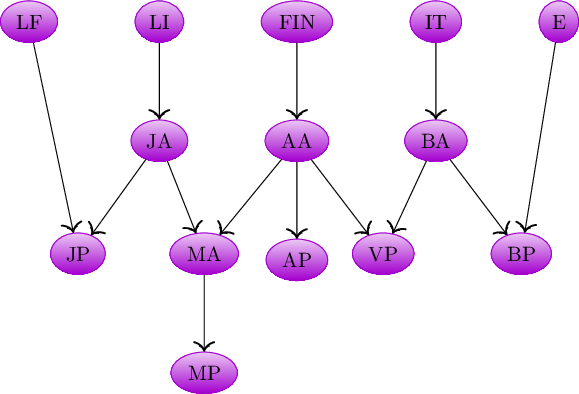
\includegraphics[width=0.8\textwidth]{inferenciasfactor/ComplicadaPedro.png}
 \caption{Gráfica con las relaciones de dependencia condicional del problema de la Fiesta de Pedro.  El significado de los nodos y las distribuciones de probabilidad correspondientes se pueden encontrar entre los textos del curso.}\label{Fig:GrafPedro}
\end{figure}


\section{Desarrollo}

Para resolver los ejercicios siguientes deberás utilizar la clase que programaste en la práctica Factores, por lo que será necesario que la entregues empaquetada en esta práctica también; si deseas hacer correcciones es un buen momento para incluirlas.

\subsection{Requisitos y resultados}

Para las instrucciones siguientes asumiremos que el código está en \code{Python}.  Si alguien decidió trabajar en otro lenguaje deberá consultar directamente con el ayudante del curso y adaptar las indicaciones a las convenciones del lenguaje elegido.

\begin{enumerate}
 \item Para esta práctica deberás entregar dos archivos:
 \begin{enumerate}
  \item \code{Factor.py}.  Es el código de la práctica anterior y será necesario para ejecutar esta.
  \item \code{PedroFactor.py}.  En este \textit{script} colocarás las funciones para resolver los problemas indicados.  Cada función que programes deberá:
  \begin{enumerate}
   \item Imprimir al inicio cuál es la \emph{consulta} (probabilidad) que está realizando.
   \item Los factores con resultados intermedios relevantes.  Antes de imprimir el factor, imprime su significado.  Por ejemplo: $P(ma|AP,VP)$, $P(MA,mp)$ ó $P(MA,JA)P(LI|bp)$.
   \item El resultado final, igualmente con algún formato que lo haga resaltar de las demás operaciones.
  \end{enumerate}
  Al final, en la sección \code{if \_\_name\_\_=='\_\_main\_\_':} mandar ejecutar todas las funciones mostrando tus resultados para cada ejercicio.
 \end{enumerate}
\end{enumerate}

\textbf{Notación:} Para abreviar sumas/marginalizaciones sucesivas, se utilizará la siguiente abreviatura:
\begin{align*}
 \sum_{A,B,C} &= \sum_A \sum_B \sum_C f(A,B,C)
\end{align*}


Las tareas que debes realizar son las siguientes:
\begin{enumerate}
 \item Crea todas las variables correspondientes a las variables aleatorias de la fiesta de Pedro como variables globales del \textit{script}.
 
 \item Crea todos los factores correspondientes a las distribuciones de probabilidad, también como variables globales.
 
 \item Crea una función por cada ecuación, donde resuelvas directamente la traducción de las operaciones siguientes, en el orden en el que están especificadas.  Para cada versión imprime el número de renglones que tienen tus factores después de cada multiplicación y marginalización. Observa que, al final, todas deben dar el mismo resultado
 \begin{align}
  P(VP,BP) =& \sum_{AA,BA,FIN,IT,E} P(VP|AA,BA)P(BP|BA,E)P(AA|FIN) \\
            & P(BA|IT)P(FIN)P(IT)P(E) \nonumber \\
  P(VP,BP) =& \sum_{AA,BA} P(VP|AA,BA)\sum_E P(BP|BA,E)\sum_{FIN}P(AA|FIN) \\
            & \sum_{IT}P(BA|IT)P(FIN)P(IT)P(E) \nonumber \\
  P(VP,BP) =& \sum_{AA,BA} \left\lbrace P(VP|AA,BA) \left[\sum_{FIN}P(AA|FIN)P(FIN)\right] \right\rbrace \\
            & \left[\sum_E P(BP|BA,E)P(E)\right] \left[ \sum_{IT}P(BA|IT)P(IT) \right] \nonumber
 \end{align}
 
 \item Calcula la probabilidad de que María, Alicia y Víctor estén en la fiesta $P(MP,AP,VP)$.
 
 \item Calcula la probabilidad de que haya llovido el día que enviaron la invitación dado que María y Alicia estuvieron presentes.  Para ello seguirás el método siguiente.
 Recuerda que, por definición de probabilidad condicional:
 \begin{align*}
   P(LI|mp,ap) &= \frac{P(LI,mp,ap)}{P(mp,ap)}
 \end{align*}
  
 \begin{enumerate}
  \item Calcula la ecuación correspondiente para obtener $P(LI,mp,ap)$ usando la regla de la cadena para redes de Bayes.  Factorízala según sea conveniente y escribe tu resultado en los comentarios de la función de python para este ejercicio.
  
  \item Utiliza tus factores para obtener el resultado correspondiente, pero antes de multiplicar y marginalizar, manda llamar la operación \code{reducir} sobre todos los factores que contengan a $MP$ y $AP$, de modo que sólo te quedes con los renglones donde $MP=mp$ y $AP=ap$.
  
  \item Normaliza tu resultado final, esta es la probabilidad que estabas buscando.
 \end{enumerate}


\end{enumerate}
